\documentclass{article}\usepackage[]{graphicx}\usepackage[]{color}
% maxwidth is the original width if it is less than linewidth
% otherwise use linewidth (to make sure the graphics do not exceed the margin)
\makeatletter
\def\maxwidth{ %
  \ifdim\Gin@nat@width>\linewidth
    \linewidth
  \else
    \Gin@nat@width
  \fi
}
\makeatother

\definecolor{fgcolor}{rgb}{0.345, 0.345, 0.345}
\newcommand{\hlnum}[1]{\textcolor[rgb]{0.686,0.059,0.569}{#1}}%
\newcommand{\hlstr}[1]{\textcolor[rgb]{0.192,0.494,0.8}{#1}}%
\newcommand{\hlcom}[1]{\textcolor[rgb]{0.678,0.584,0.686}{\textit{#1}}}%
\newcommand{\hlopt}[1]{\textcolor[rgb]{0,0,0}{#1}}%
\newcommand{\hlstd}[1]{\textcolor[rgb]{0.345,0.345,0.345}{#1}}%
\newcommand{\hlkwa}[1]{\textcolor[rgb]{0.161,0.373,0.58}{\textbf{#1}}}%
\newcommand{\hlkwb}[1]{\textcolor[rgb]{0.69,0.353,0.396}{#1}}%
\newcommand{\hlkwc}[1]{\textcolor[rgb]{0.333,0.667,0.333}{#1}}%
\newcommand{\hlkwd}[1]{\textcolor[rgb]{0.737,0.353,0.396}{\textbf{#1}}}%
\let\hlipl\hlkwb

\usepackage{framed}
\makeatletter
\newenvironment{kframe}{%
 \def\at@end@of@kframe{}%
 \ifinner\ifhmode%
  \def\at@end@of@kframe{\end{minipage}}%
  \begin{minipage}{\columnwidth}%
 \fi\fi%
 \def\FrameCommand##1{\hskip\@totalleftmargin \hskip-\fboxsep
 \colorbox{shadecolor}{##1}\hskip-\fboxsep
     % There is no \\@totalrightmargin, so:
     \hskip-\linewidth \hskip-\@totalleftmargin \hskip\columnwidth}%
 \MakeFramed {\advance\hsize-\width
   \@totalleftmargin\z@ \linewidth\hsize
   \@setminipage}}%
 {\par\unskip\endMakeFramed%
 \at@end@of@kframe}
\makeatother

\definecolor{shadecolor}{rgb}{.97, .97, .97}
\definecolor{messagecolor}{rgb}{0, 0, 0}
\definecolor{warningcolor}{rgb}{1, 0, 1}
\definecolor{errorcolor}{rgb}{1, 0, 0}
\newenvironment{knitrout}{}{} % an empty environment to be redefined in TeX

\usepackage{alltt}

\usepackage{float}

% Set the margins on the page to not be so large
\addtolength{\oddsidemargin}{-.875in}
\addtolength{\evensidemargin}{-.875in}
\addtolength{\textwidth}{1.75in}
\addtolength{\topmargin}{-.875in}
\addtolength{\textheight}{1.75in}

% Take off page numbering
\pagenumbering{gobble}
\IfFileExists{upquote.sty}{\usepackage{upquote}}{}
\begin{document}

\title{%
  3.3.1 - R: Influential Observations and Outliers \\
  \smallskip
  \large Stat 5100: Dr. Bean
}
\date{}

\maketitle

\textbf{Example:} Data collected on 50 countries relevant to a cross-sectional study of a life-cycle savings hypothesis, which states that the response variable

\begin{itemize}
  \item SavRatio: aggregate personal saving divided by disposable income
\end{itemize}

can be explained by the following four predictor variables:

\begin{itemize}
  \item AvIncome: per-capita disposable income, in USD (yearly average over decade)
  \item GrowRate: percentage growth rate in per-capita disposable income (over decade)
  \item PopU15: percentage of the population less than 15 years old (yearly average over decade)
  \item PopO75: percentage of the population over 75 years old (yearly average over decade)
\end{itemize}

The decade is 1960-1970.  These data are published in section 2.2 of Regression Diagnostics: Identifying Influential Data and Sources of Collinearity (1980) by Belsley, Kuh, and Welsch (limited excerpt available through Google books).

\begin{knitrout}
\definecolor{shadecolor}{rgb}{0.969, 0.969, 0.969}\color{fgcolor}\begin{kframe}
\begin{alltt}
\hlcom{# Load in and take a look at the data}
\hlkwd{library}\hlstd{(stat5100)}
\hlkwd{data}\hlstd{(savings)}

\hlcom{# Create a regression model to predict SavRatio}
\hlstd{savings_lm} \hlkwb{<-} \hlkwd{lm}\hlstd{(SavingsRatio} \hlopt{~} \hlstd{PctPopU15} \hlopt{+} \hlstd{PctPopO75} \hlopt{+} \hlstd{AverageIncome} \hlopt{+} \hlstd{GrowthRate,}
                 \hlkwc{data} \hlstd{= savings)}

\hlcom{# Look at some basic visual assumptions}
\hlstd{stat5100}\hlopt{::}\hlkwd{visual_assumptions}\hlstd{(savings_lm)}
\end{alltt}
\end{kframe}

{\centering 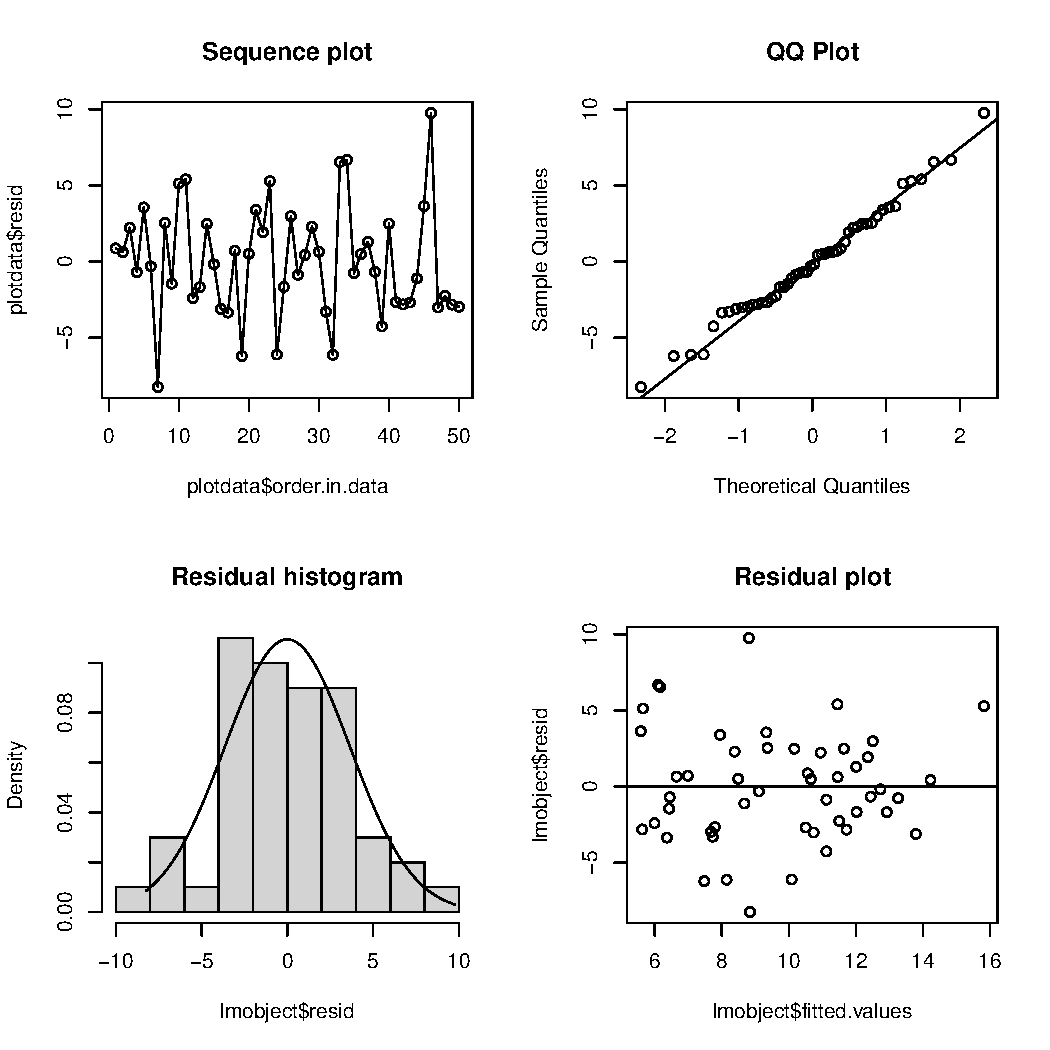
\includegraphics[width=0.4\textwidth]{figure/unnamed-chunk-1-1} 

}


\begin{kframe}\begin{alltt}
\hlcom{# Numerical assumptions}
\hlstd{stat5100}\hlopt{::}\hlkwd{brown_forsythe_lm}\hlstd{(savings_lm)}
\end{alltt}
\begin{verbatim}
## [1] "Brown-forsythe test for constant variance in the residuals:"
## [1] "T-statistic: 1.9704, p-value: 0.0546"
\end{verbatim}
\begin{alltt}
\hlstd{stat5100}\hlopt{::}\hlkwd{cor_normality_lm}\hlstd{(savings_lm)}
\end{alltt}
\begin{verbatim}
## Correlation test of normality:
##                   resid expected_norm
## resid         1.0000000     0.9925168
## expected_norm 0.9925168     1.0000000
## 
## Total observations: 50
## Make sure to consult with table B.6 for your final result.
\end{verbatim}
\end{kframe}
\end{knitrout}

\subsubsection*{Look at some diagnostics for influential observations and outliers}

\begin{knitrout}
\definecolor{shadecolor}{rgb}{0.969, 0.969, 0.969}\color{fgcolor}\begin{kframe}
\begin{alltt}
\hlcom{# Cook's D Chart}
\hlstd{olsrr}\hlopt{::}\hlkwd{ols_plot_cooksd_chart}\hlstd{(savings_lm)}
\end{alltt}
\end{kframe}

{\centering 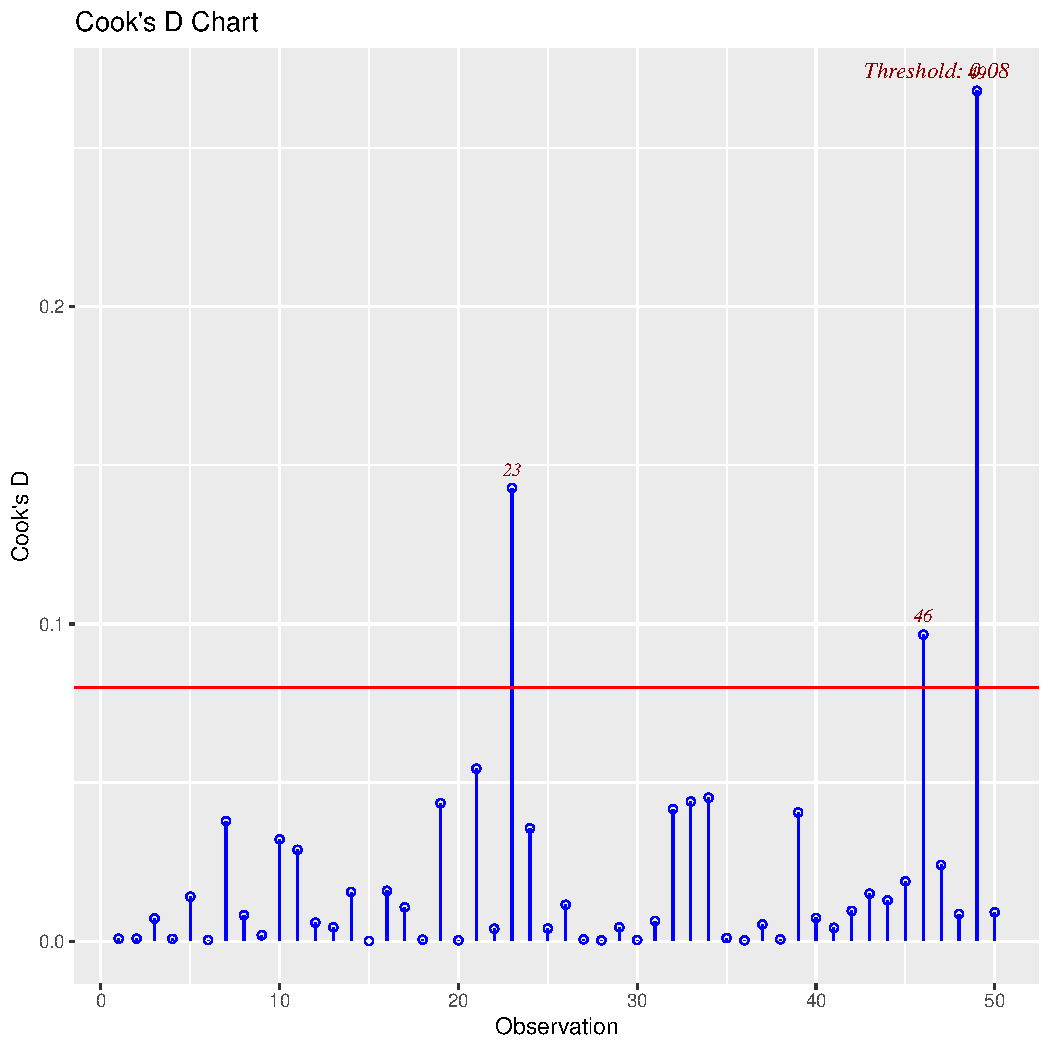
\includegraphics[width=0.5\textwidth]{figure/unnamed-chunk-2-1} 

}


\begin{kframe}\begin{alltt}
\hlcom{# The output above for Cook's D doesn't tell us which names belong to the numbers}
\hlcom{# in the graph. We can find them by indexing the country vector inside savings:}
\hlstd{savings}\hlopt{$}\hlstd{Country[}\hlkwd{c}\hlstd{(}\hlnum{23}\hlstd{,} \hlnum{46}\hlstd{,} \hlnum{49}\hlstd{)]}
\end{alltt}
\begin{verbatim}
## [1] "Japan"  "Zambia" "Libya"
\end{verbatim}
\begin{alltt}
\hlcom{# Which tells us that countries Japan, Zambia, and Libya strongly influenced}
\hlcom{# the fitted values of the model.}
\end{alltt}
\end{kframe}
\end{knitrout}

\begin{knitrout}
\definecolor{shadecolor}{rgb}{0.969, 0.969, 0.969}\color{fgcolor}\begin{kframe}
\begin{alltt}
\hlcom{# Outlier and Leverage Diagnostics}
\hlstd{olsrr}\hlopt{::}\hlkwd{ols_plot_resid_lev}\hlstd{(savings_lm)}
\end{alltt}
\end{kframe}

{\centering 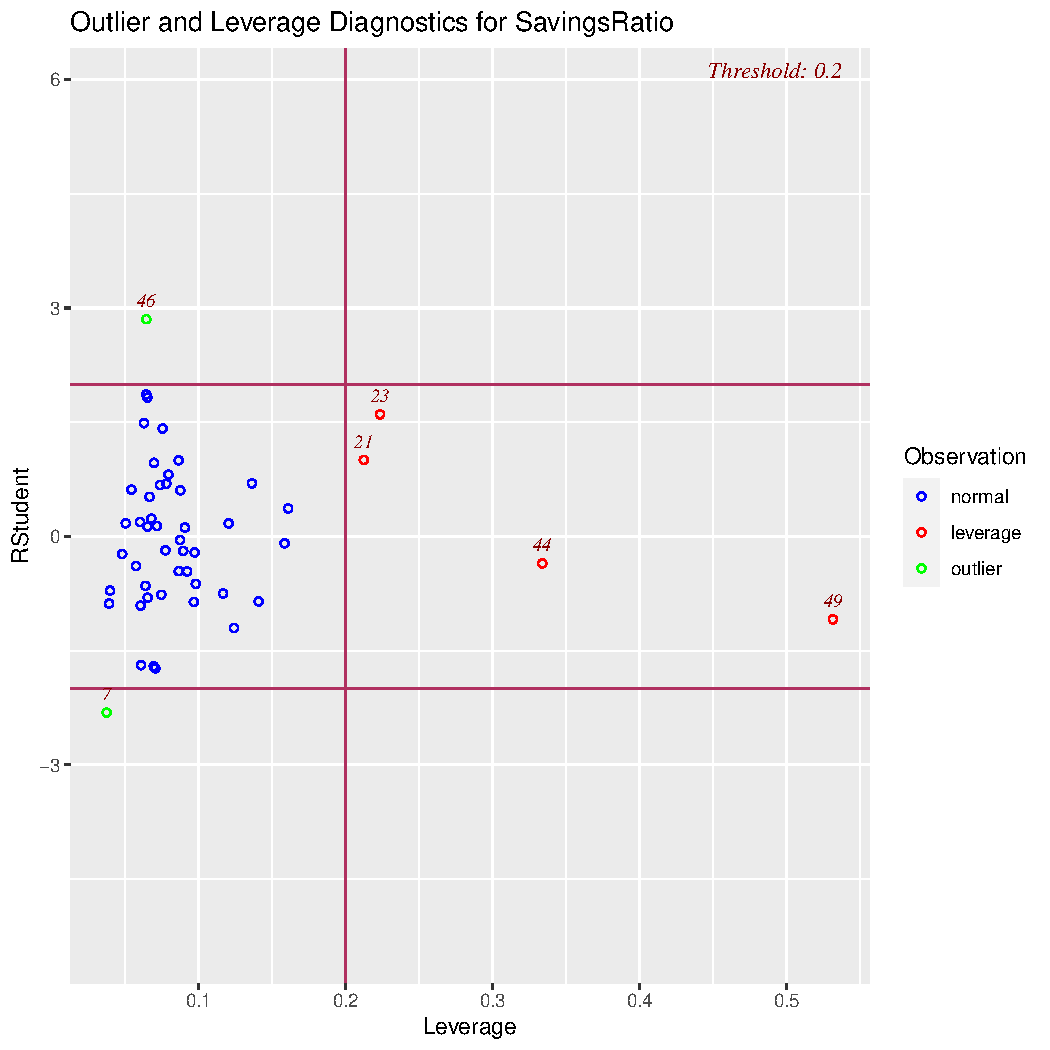
\includegraphics[width=0.6\textwidth]{figure/unnamed-chunk-3-1} 

}


\begin{kframe}\begin{alltt}
\hlcom{# Once again we can find the names by indexing:}
\hlstd{savings}\hlopt{$}\hlstd{Country[}\hlkwd{c}\hlstd{(}\hlnum{7}\hlstd{,} \hlnum{46}\hlstd{)]} \hlcom{# Outliers}
\end{alltt}
\begin{verbatim}
## [1] "Chile"  "Zambia"
\end{verbatim}
\begin{alltt}
\hlstd{savings}\hlopt{$}\hlstd{Country[}\hlkwd{c}\hlstd{(}\hlnum{23}\hlstd{,} \hlnum{21}\hlstd{,} \hlnum{44}\hlstd{,} \hlnum{49}\hlstd{)]} \hlcom{# Leverage}
\end{alltt}
\begin{verbatim}
## [1] "Japan"         "Ireland"       "United States" "Libya"
\end{verbatim}
\end{kframe}
\end{knitrout}

\begin{knitrout}
\definecolor{shadecolor}{rgb}{0.969, 0.969, 0.969}\color{fgcolor}\begin{kframe}
\begin{alltt}
\hlcom{# DFFITs plot:}
\hlstd{olsrr}\hlopt{::}\hlkwd{ols_plot_dffits}\hlstd{(savings_lm)}
\end{alltt}
\end{kframe}

{\centering 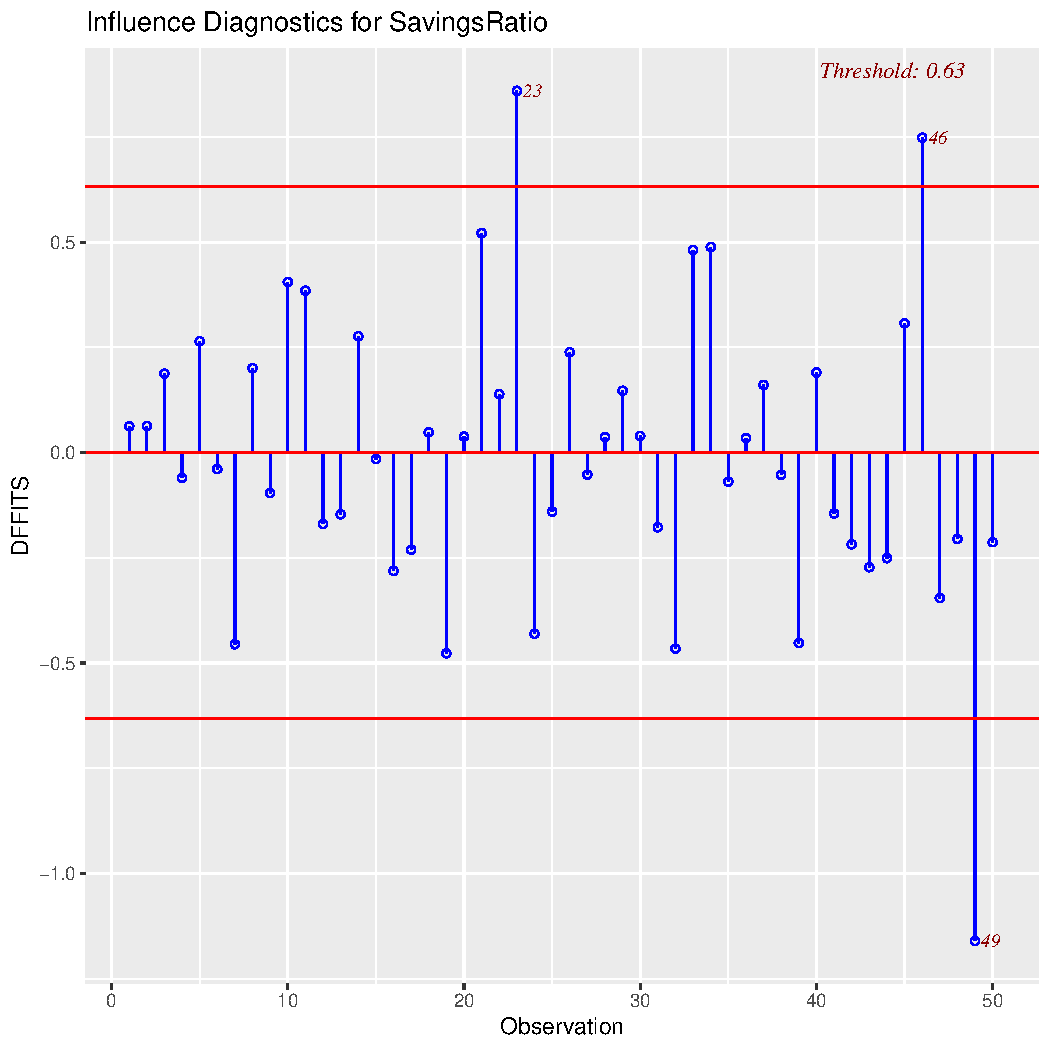
\includegraphics[width=0.5\textwidth]{figure/unnamed-chunk-4-1} 

}



\end{knitrout}

\begin{knitrout}
\definecolor{shadecolor}{rgb}{0.969, 0.969, 0.969}\color{fgcolor}\begin{kframe}
\begin{alltt}
\hlcom{# DFBETAs panel:}
\hlstd{olsrr}\hlopt{::}\hlkwd{ols_plot_dfbetas}\hlstd{(savings_lm)}
\end{alltt}
\end{kframe}

{\centering 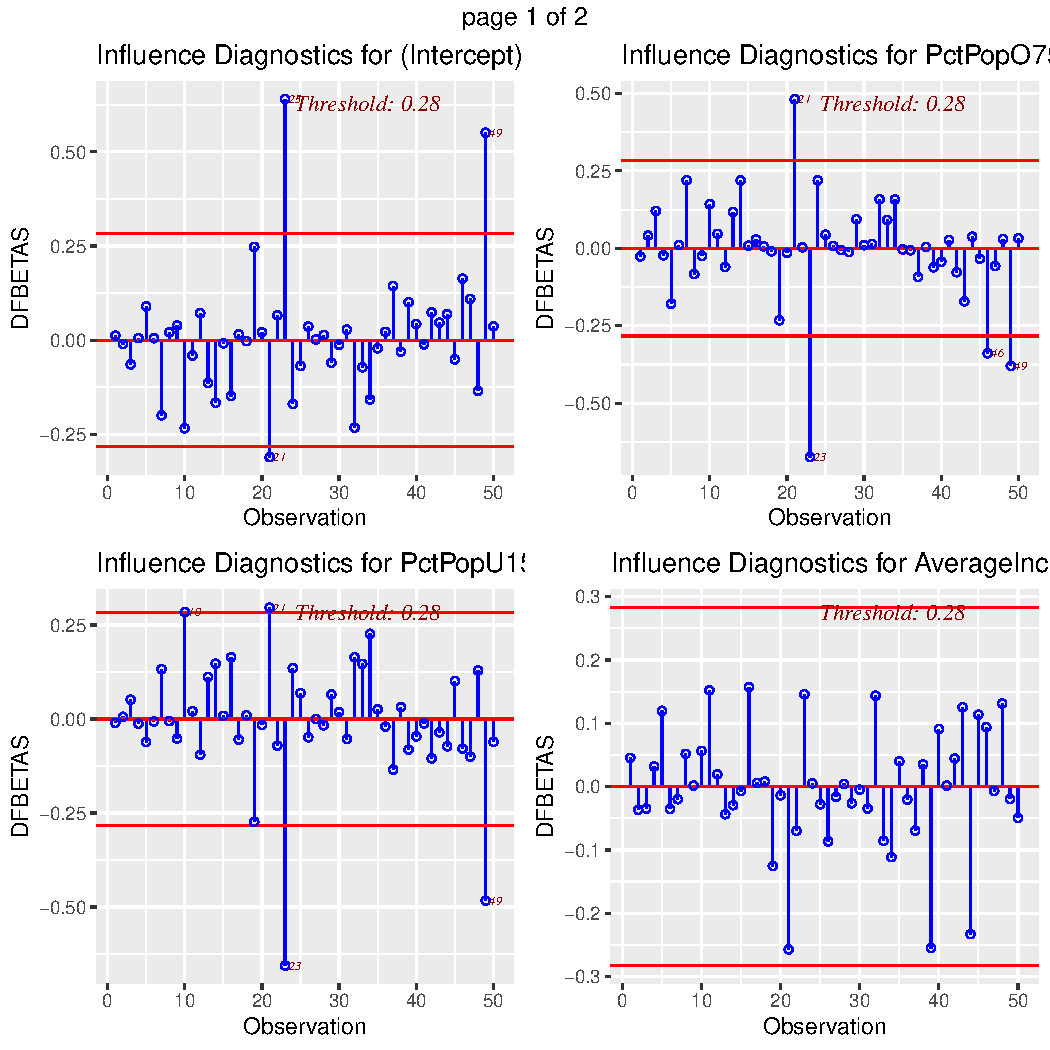
\includegraphics[width=0.6\textwidth]{figure/unnamed-chunk-5-1} 

}




{\centering 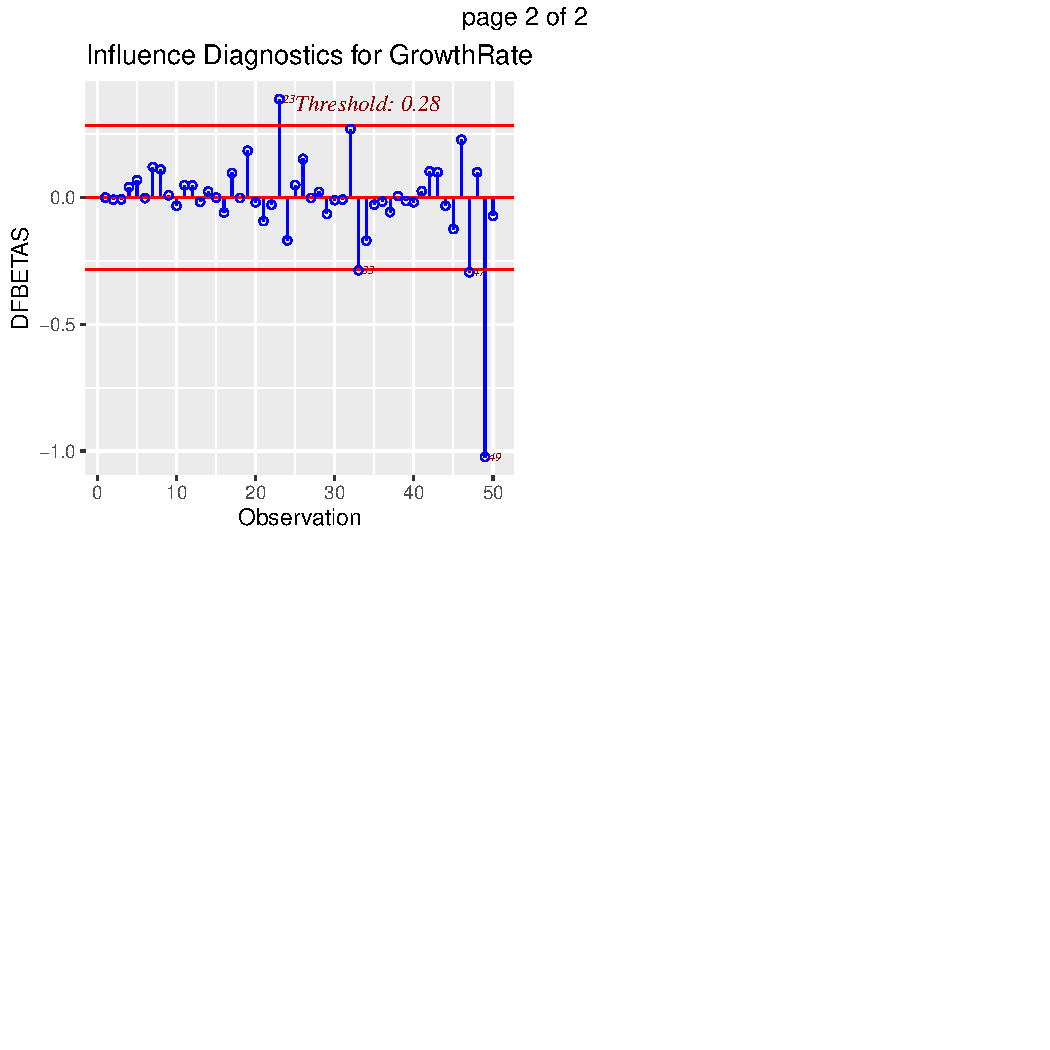
\includegraphics[width=0.6\textwidth]{figure/unnamed-chunk-5-2} 

}



\end{knitrout}

\newpage

\subsubsection*{Alternative thresholds for influential observations and outlier diagnostics}

\begin{knitrout}
\definecolor{shadecolor}{rgb}{0.969, 0.969, 0.969}\color{fgcolor}\begin{kframe}
\begin{alltt}
\hlstd{p} \hlkwb{<-} \hlnum{5} \hlcom{# Number of beta parameters, including intercept}
\hlstd{n} \hlkwb{<-} \hlnum{50} \hlcom{# Sample size}

\hlstd{cooks_d_simple} \hlkwb{<-} \hlnum{4} \hlopt{/} \hlstd{n}
\hlstd{cooks_d_10} \hlkwb{<-} \hlkwd{qf}\hlstd{(}\hlnum{0.10}\hlstd{, p, n}\hlopt{-}\hlstd{p)}
\hlstd{cooks_d_20} \hlkwb{<-} \hlkwd{qf}\hlstd{(}\hlnum{0.20}\hlstd{, p, n}\hlopt{-}\hlstd{p)}
\hlstd{cooks_d_50} \hlkwb{<-} \hlkwd{qf}\hlstd{(}\hlnum{0.50}\hlstd{, p, n}\hlopt{-}\hlstd{p)}

\hlstd{rstudent_95} \hlkwb{<-} \hlkwd{qt}\hlstd{(}\hlnum{1} \hlopt{-} \hlnum{0.05}\hlopt{/}\hlnum{2}\hlstd{, n}\hlopt{-}\hlstd{p)}
\hlstd{rstudent_95_bonf} \hlkwb{<-} \hlkwd{qt}\hlstd{(}\hlnum{1} \hlopt{-} \hlnum{0.05}\hlopt{/}\hlstd{(}\hlnum{2}\hlopt{*}\hlstd{n), n}\hlopt{-}\hlstd{p)}

\hlstd{leverage_2} \hlkwb{<-} \hlnum{2} \hlopt{*} \hlstd{p}\hlopt{/}\hlstd{n}
\hlstd{leverage_3} \hlkwb{<-} \hlnum{3} \hlopt{*} \hlstd{p}\hlopt{/}\hlstd{n}

\hlcom{# If we had n less than 30, then we should set both DFBETAS and DFFITS to 1.}
\hlstd{DFBETAS} \hlkwb{=} \hlnum{2}\hlopt{/}\hlstd{(n}\hlopt{^}\hlnum{0.5}\hlstd{)}
\hlstd{DFFITS} \hlkwb{=} \hlnum{2}\hlopt{*}\hlstd{(p}\hlopt{/}\hlstd{n)}\hlopt{^}\hlnum{0.5}

\hlcom{# Look at all the alternative thresholds:}
\hlstd{thresholds} \hlkwb{<-} \hlkwd{data.frame}\hlstd{(cooks_d_simple, cooks_d_10, cooks_d_20, cooks_d_50, rstudent_95,}
                \hlstd{rstudent_95_bonf, leverage_2, leverage_3, DFBETAS, DFFITS)}
\hlstd{thresholds}
\end{alltt}
\begin{verbatim}
##   cooks_d_simple cooks_d_10 cooks_d_20 cooks_d_50 rstudent_95 rstudent_95_bonf
## 1           0.08  0.3172927   0.465266  0.8834915    2.014103         3.520251
##   leverage_2 leverage_3   DFBETAS    DFFITS
## 1        0.2        0.3 0.2828427 0.6324555
\end{verbatim}
\end{kframe}
\end{knitrout}

\newpage

\subsubsection*{Look closely at the distribution of predictors and the suspect observations}

\begin{knitrout}
\definecolor{shadecolor}{rgb}{0.969, 0.969, 0.969}\color{fgcolor}\begin{kframe}
\begin{alltt}
\hlcom{# Tile 4 histograms together of the four predictors}
\hlkwd{par}\hlstd{(}\hlkwc{mfrow} \hlstd{=} \hlkwd{c}\hlstd{(}\hlnum{2}\hlstd{,} \hlnum{2}\hlstd{))}
\hlkwd{hist}\hlstd{(savings}\hlopt{$}\hlstd{PctPopU15,} \hlkwc{main} \hlstd{=} \hlstr{"Distribution of PctPopU15"}\hlstd{,} \hlkwc{xlab} \hlstd{=} \hlstr{"PctPopU15"}\hlstd{)}
\hlkwd{hist}\hlstd{(savings}\hlopt{$}\hlstd{PctPopO75,} \hlkwc{main} \hlstd{=} \hlstr{"Distribution of PctPopO75"}\hlstd{,} \hlkwc{xlab} \hlstd{=} \hlstr{"PctPopO75"}\hlstd{)}
\hlkwd{hist}\hlstd{(savings}\hlopt{$}\hlstd{AverageIncome,} \hlkwc{main} \hlstd{=} \hlstr{"Distribution of Average Income"}\hlstd{,}
     \hlkwc{xlab} \hlstd{=} \hlstr{"Average Income"}\hlstd{)}
\hlkwd{hist}\hlstd{(savings}\hlopt{$}\hlstd{GrowthRate,} \hlkwc{main} \hlstd{=} \hlstr{"Distribution of Growth Rate"}\hlstd{,}
     \hlkwc{xlab} \hlstd{=} \hlstr{"Growth Rate"}\hlstd{)}
\end{alltt}
\end{kframe}

{\centering 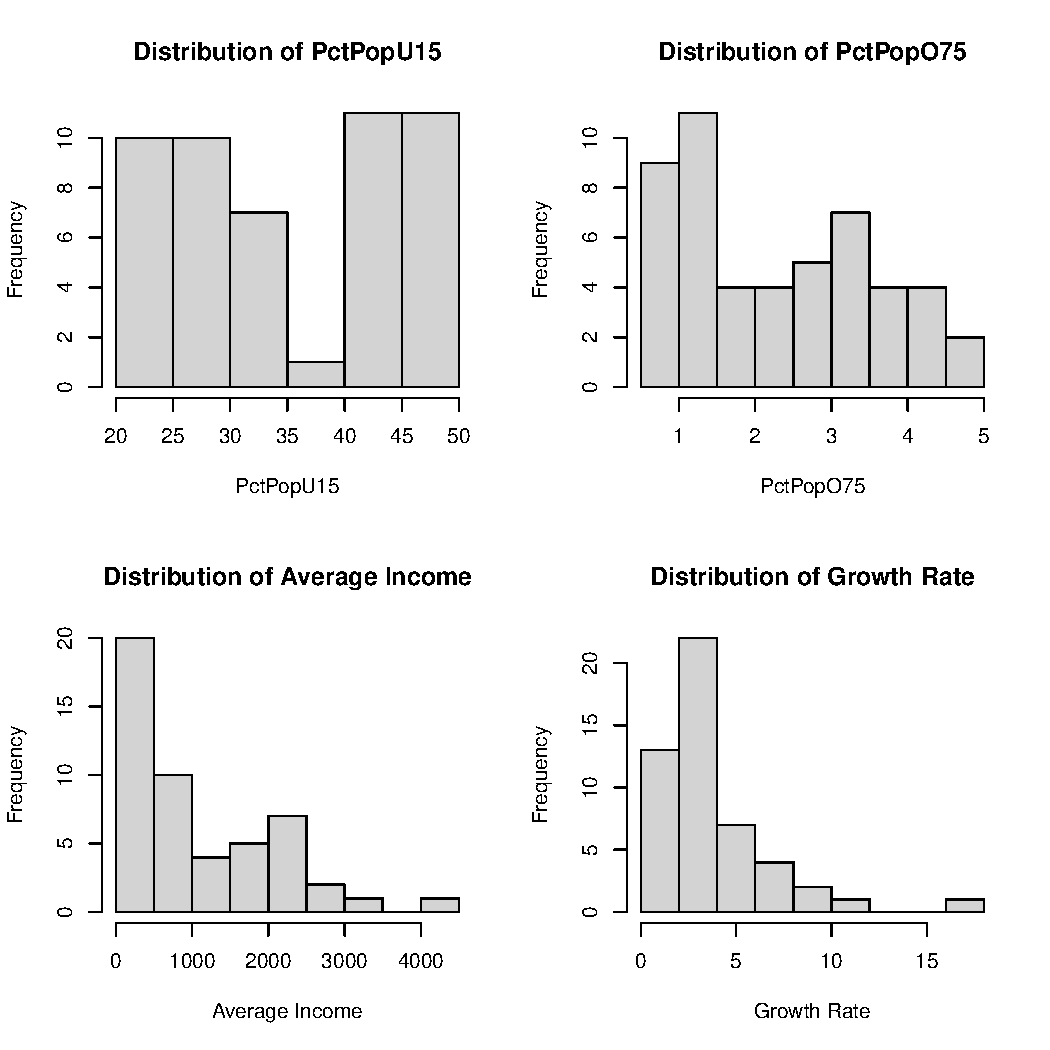
\includegraphics[width=0.6\textwidth]{figure/unnamed-chunk-7-1} 

}


\begin{kframe}\begin{alltt}
\hlcom{# Reset plot to just one graph per plot}
\hlkwd{par}\hlstd{(}\hlkwc{mfrow} \hlstd{=} \hlkwd{c}\hlstd{(}\hlnum{1}\hlstd{,} \hlnum{1}\hlstd{))}

\hlcom{# Look at the suspect observations (previously identified influential points}
\hlcom{# and outliers)}

\hlstd{suspect_observations} \hlkwb{<-} \hlstd{savings[savings}\hlopt{$}\hlstd{Country} \hlopt \hlkwd{c}\hlstd{(}\hlstr{"Ireland"}\hlstd{,} \hlstr{"Japan"}\hlstd{,}
                                                       \hlstr{"United States"}\hlstd{,} \hlstr{"Libya"}\hlstd{,}
                                                       \hlstr{"Zambia"}\hlstd{), ]}
\hlstd{suspect_observations}
\end{alltt}
\begin{verbatim}
##          Country SavingsRatio PctPopU15 PctPopO75 AverageIncome GrowthRate
## 21       Ireland        11.34     31.16      4.19       1139.95       2.99
## 23         Japan        21.10     27.01      1.91       1257.28       8.21
## 44 United States         7.56     29.81      3.43       4001.89       2.45
## 46        Zambia        18.56     45.25      0.56        138.33       5.14
## 49         Libya         8.89     43.69      2.07        123.58      16.71
\end{verbatim}
\end{kframe}
\end{knitrout}

\newpage

\subsubsection*{What are some possible remedial measures for this data?}

\begin{enumerate}
  \item Drop Japan
  \begin{itemize}
    \item PopU15 and PopO75 don't match the profile (influential but not outliers)
  \end{itemize}

  \item Take a log transform of AverageIncome and GrowthRate
  \begin{itemize}
    \item Both distributions are skewed right
    \item The extreme observations in each is a suspect observation (United States for AverageIncome, and Libya for GrowthRate)
  \end{itemize}
\end{enumerate}

\begin{knitrout}
\definecolor{shadecolor}{rgb}{0.969, 0.969, 0.969}\color{fgcolor}\begin{kframe}
\begin{alltt}
\hlcom{# Create new dataset, fit regression model, and then check assumptions}
\hlstd{new_savings} \hlkwb{<-} \hlstd{savings}
\hlstd{new_savings} \hlkwb{<-} \hlstd{new_savings[new_savings}\hlopt{$}\hlstd{Country} \hlopt{!=} \hlstr{"Japan"}\hlstd{, ]}
\hlstd{new_savings} \hlkwb{<-} \hlkwd{cbind}\hlstd{(new_savings,} \hlkwc{logAverageIncome} \hlstd{=} \hlkwd{log}\hlstd{(new_savings}\hlopt{$}\hlstd{AverageIncome),}
                     \hlkwc{logGrowthRate} \hlstd{=} \hlkwd{log}\hlstd{(new_savings}\hlopt{$}\hlstd{GrowthRate))}

\hlstd{new_savings_lm} \hlkwb{<-} \hlkwd{lm}\hlstd{(SavingsRatio} \hlopt{~} \hlstd{PctPopU15} \hlopt{+} \hlstd{PctPopO75} \hlopt{+} \hlstd{logAverageIncome} \hlopt{+}
                       \hlstd{logGrowthRate,} \hlkwc{data} \hlstd{= new_savings)}

\hlkwd{summary}\hlstd{(new_savings_lm)}
\end{alltt}
\begin{verbatim}
## 
## Call:
## lm(formula = SavingsRatio ~ PctPopU15 + PctPopO75 + logAverageIncome + 
##     logGrowthRate, data = new_savings)
## 
## Residuals:
##     Min      1Q  Median      3Q     Max 
## -7.9240 -2.3669  0.0355  2.1058  9.3683 
## 
## Coefficients:
##                  Estimate Std. Error t value Pr(>|t|)  
## (Intercept)       26.2512    10.5263   2.494   0.0165 *
## PctPopU15         -0.3384     0.1579  -2.143   0.0377 *
## PctPopO75         -0.6856     1.1357  -0.604   0.5492  
## logAverageIncome  -0.7186     0.9749  -0.737   0.4650  
## logGrowthRate      1.3304     0.7253   1.834   0.0734 .
## ---
## Signif. codes:  0 '***' 0.001 '**' 0.01 '*' 0.05 '.' 0.1 ' ' 1
## 
## Residual standard error: 3.716 on 44 degrees of freedom
## Multiple R-squared:  0.2855,	Adjusted R-squared:  0.2206 
## F-statistic: 4.396 on 4 and 44 DF,  p-value: 0.004465
\end{verbatim}
\begin{alltt}
\hlstd{stat5100}\hlopt{::}\hlkwd{visual_assumptions}\hlstd{(new_savings_lm)}
\end{alltt}
\end{kframe}

{\centering 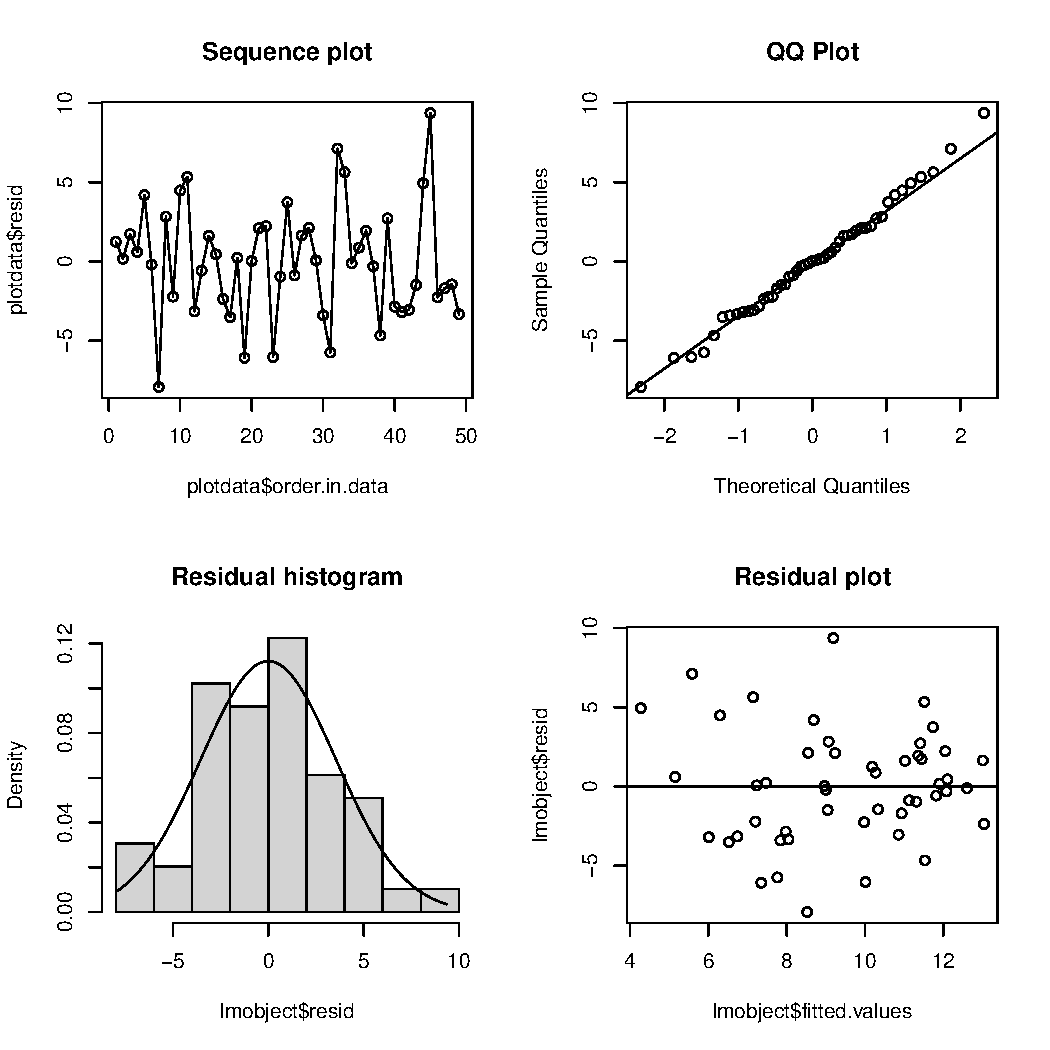
\includegraphics[width=0.6\textwidth]{figure/unnamed-chunk-8-1} 

}



\end{knitrout}

\begin{knitrout}
\definecolor{shadecolor}{rgb}{0.969, 0.969, 0.969}\color{fgcolor}\begin{kframe}
\begin{alltt}
\hlcom{# Numerical assumptions}
\hlstd{stat5100}\hlopt{::}\hlkwd{brown_forsythe_lm}\hlstd{(new_savings_lm)}
\end{alltt}
\begin{verbatim}
## [1] "Brown-forsythe test for constant variance in the residuals:"
## [1] "T-statistic: 2.4334, p-value: 0.0188"
\end{verbatim}
\begin{alltt}
\hlstd{stat5100}\hlopt{::}\hlkwd{cor_normality_lm}\hlstd{(new_savings_lm)}
\end{alltt}
\begin{verbatim}
## Correlation test of normality:
##                   resid expected_norm
## resid         1.0000000     0.9951555
## expected_norm 0.9951555     1.0000000
## 
## Total observations: 49
## Make sure to consult with table B.6 for your final result.
\end{verbatim}
\end{kframe}
\end{knitrout}

\newpage

\begin{knitrout}
\definecolor{shadecolor}{rgb}{0.969, 0.969, 0.969}\color{fgcolor}\begin{kframe}
\begin{alltt}
\hlcom{# Check a few influential observation diagnostics}
\hlcom{# ------------------------------}
\hlcom{# Cook's D and Residual / Leverage plot}
\hlstd{olsrr}\hlopt{::}\hlkwd{ols_plot_cooksd_chart}\hlstd{(new_savings_lm)}
\hlstd{olsrr}\hlopt{::}\hlkwd{ols_plot_resid_lev}\hlstd{(new_savings_lm)}
\end{alltt}
\end{kframe}

{\centering 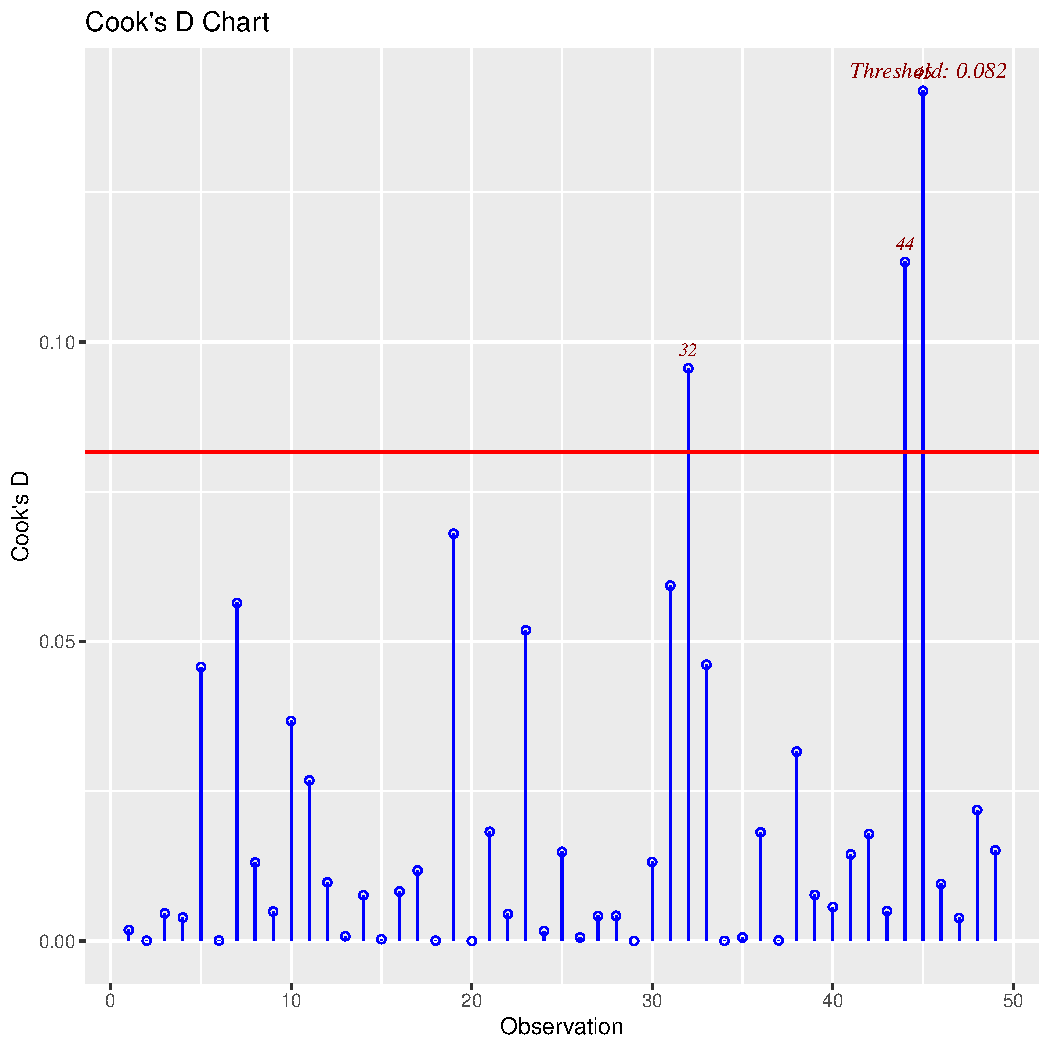
\includegraphics[width=0.45\textwidth]{figure/unnamed-chunk-10-1} 
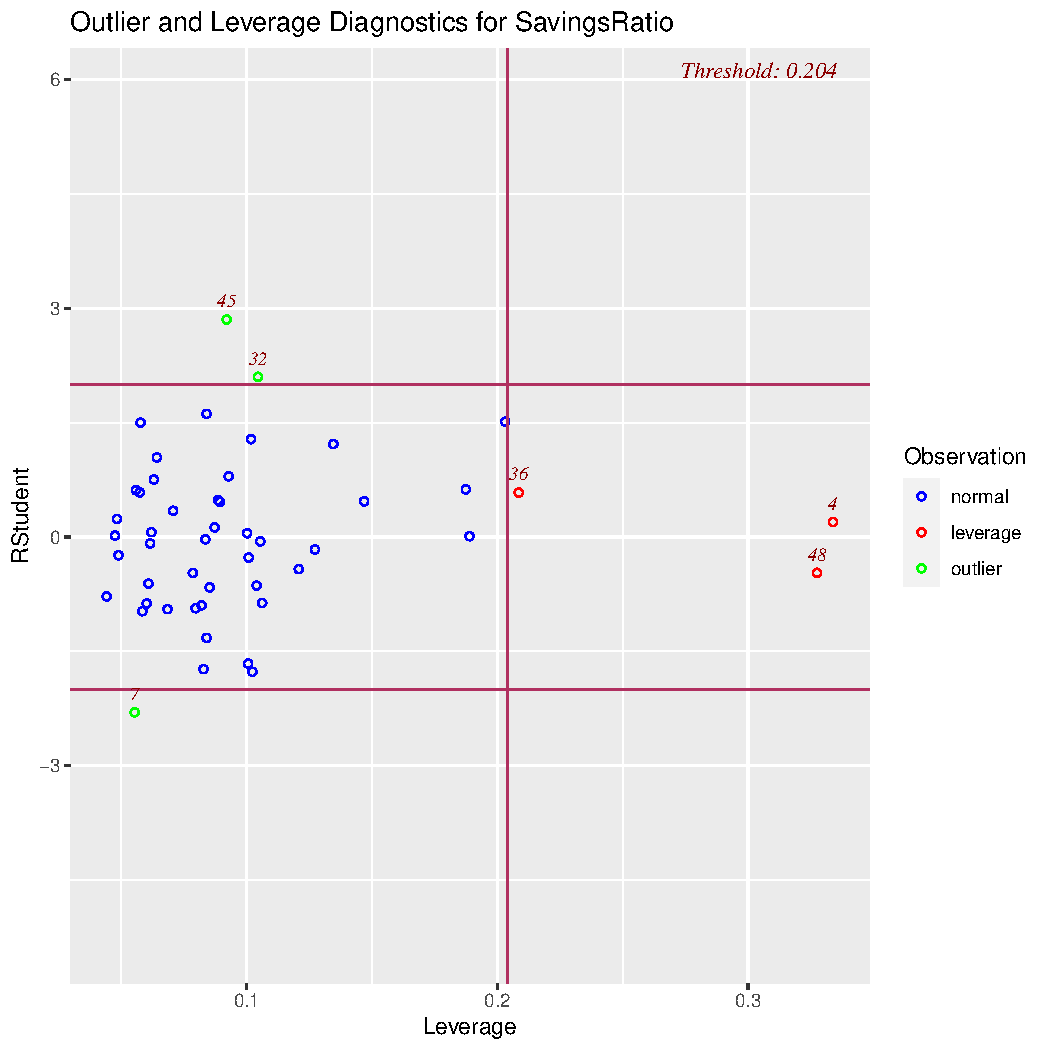
\includegraphics[width=0.45\textwidth]{figure/unnamed-chunk-10-2} 

}



\end{knitrout}

\begin{knitrout}
\definecolor{shadecolor}{rgb}{0.969, 0.969, 0.969}\color{fgcolor}\begin{kframe}
\begin{alltt}
\hlcom{# DFFITs plot:}
\hlstd{olsrr}\hlopt{::}\hlkwd{ols_plot_dffits}\hlstd{(new_savings_lm)}
\end{alltt}
\end{kframe}

{\centering 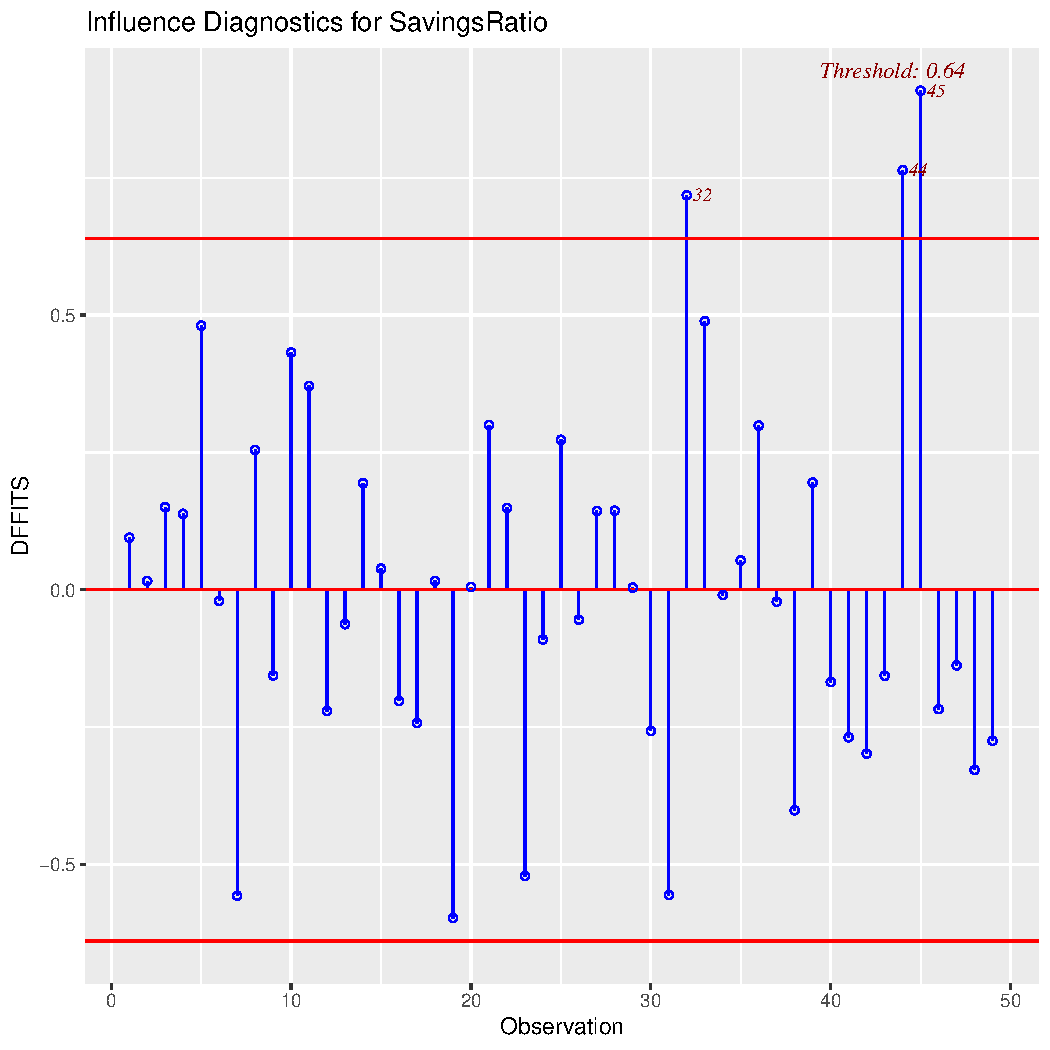
\includegraphics[width=0.45\textwidth]{figure/unnamed-chunk-11-1} 

}



\end{knitrout}

\newpage

\begin{knitrout}
\definecolor{shadecolor}{rgb}{0.969, 0.969, 0.969}\color{fgcolor}\begin{kframe}
\begin{alltt}
\hlcom{# DFBETAs panel:}
\hlstd{olsrr}\hlopt{::}\hlkwd{ols_plot_dfbetas}\hlstd{(new_savings_lm)}
\end{alltt}
\end{kframe}

{\centering 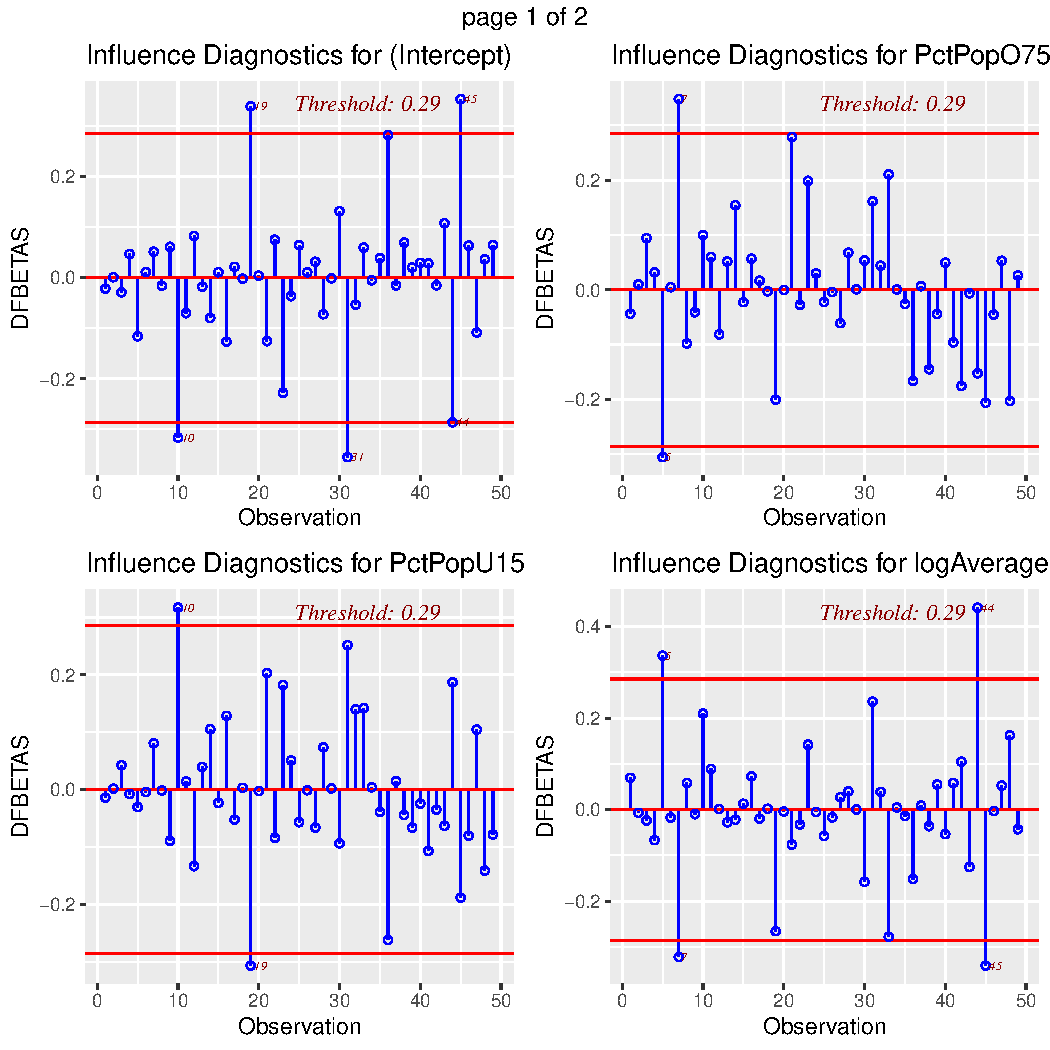
\includegraphics[width=0.6\textwidth]{figure/unnamed-chunk-12-1} 

}




{\centering 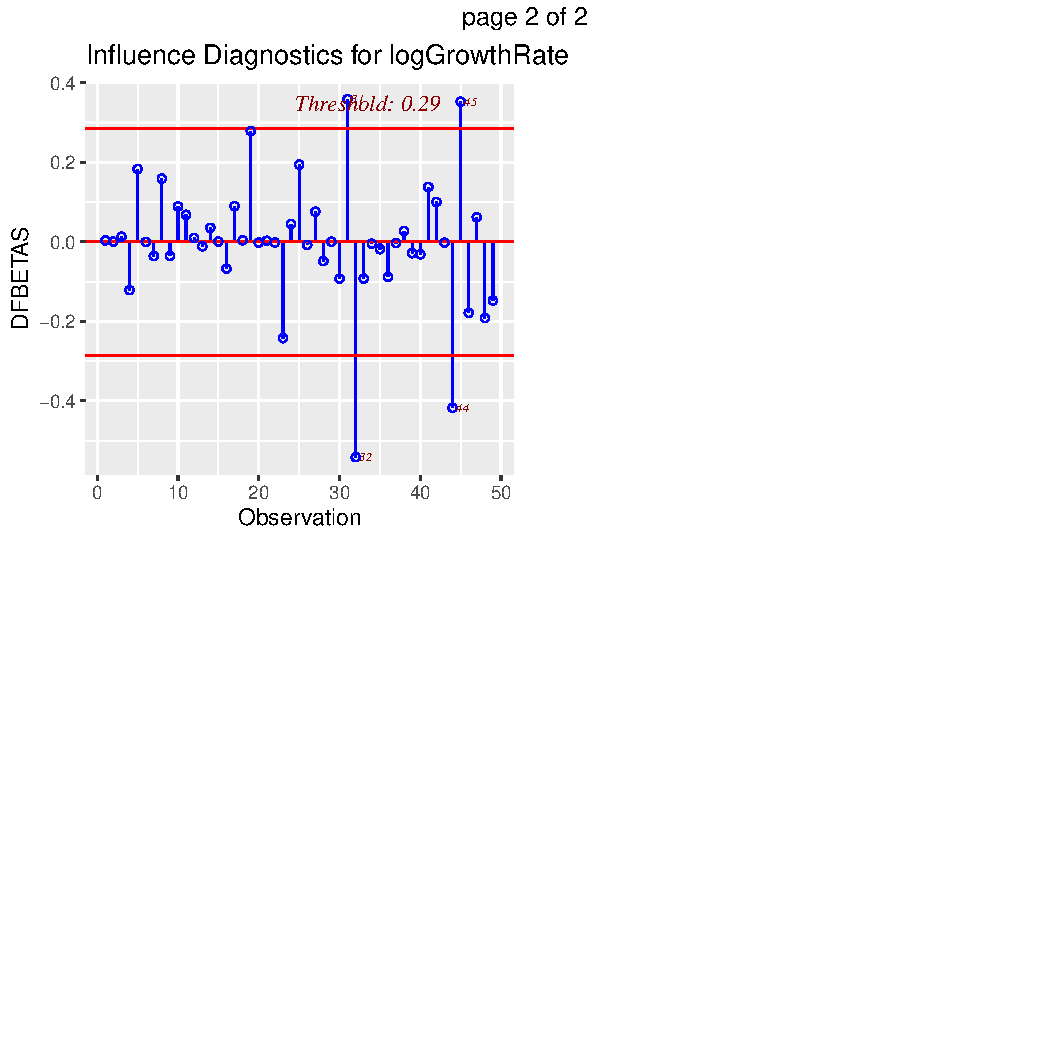
\includegraphics[width=0.6\textwidth]{figure/unnamed-chunk-12-2} 

}



\end{knitrout}

\newpage

\subsubsection*{Look at final model}

Notice that only PopU15 and logGrowthRate had $\beta$ coefficients that were significant according to the t-test. Thus, we might want to create our final model with only the two significant variables:

\begin{knitrout}
\definecolor{shadecolor}{rgb}{0.969, 0.969, 0.969}\color{fgcolor}\begin{kframe}
\begin{alltt}
\hlstd{final_savings_lm} \hlkwb{<-} \hlkwd{lm}\hlstd{(SavingsRatio} \hlopt{~} \hlstd{PctPopU15} \hlopt{+} \hlstd{logGrowthRate,} \hlkwc{data} \hlstd{= new_savings)}

\hlkwd{summary}\hlstd{(final_savings_lm)}
\end{alltt}
\begin{verbatim}
## 
## Call:
## lm(formula = SavingsRatio ~ PctPopU15 + logGrowthRate, data = new_savings)
## 
## Residuals:
##     Min      1Q  Median      3Q     Max 
## -7.9342 -2.6413  0.2752  1.8731 10.0690 
## 
## Coefficients:
##               Estimate Std. Error t value Pr(>|t|)    
## (Intercept)   14.27955    2.40166   5.946 3.49e-07 ***
## PctPopU15     -0.18046    0.05915  -3.051  0.00378 ** 
## logGrowthRate  1.45209    0.71058   2.044  0.04675 *  
## ---
## Signif. codes:  0 '***' 0.001 '**' 0.01 '*' 0.05 '.' 0.1 ' ' 1
## 
## Residual standard error: 3.69 on 46 degrees of freedom
## Multiple R-squared:  0.2632,	Adjusted R-squared:  0.2312 
## F-statistic: 8.217 on 2 and 46 DF,  p-value: 0.0008884
\end{verbatim}
\end{kframe}
\end{knitrout}


\end{document}
